\documentclass{article}
\usepackage{amsmath}
\usepackage{graphicx}
\usepackage[final]{pdfpages}
\usepackage{hyperref}

\title{MIT Math Problems}
\author{Cecilia}
\date{August 2022}

\begin{document}
\maketitle

\section*{Links}
    \begin{enumerate}
        \item \href{https://math.mit.edu/academics/undergrad/roadmaps.php}{Roadmap}
        \item \href{https://ocw.mit.edu/courses/18-700-linear-algebra-fall-2013/}{Linear Algebra}
        \begin{enumerate}
            \item \hyperlink{LinearAlgebra-ProblemSet1.1}{ProblemSet1}
            \item \hyperlink{LinearAlgebra-ProblemSet2.1}{ProblemSet2}
            \item \hyperlink{LinearAlgebra-ProblemSet3.1}{ProblemSet3}
            \item \hyperlink{LinearAlgebra-ProblemSet4.1}{ProblemSet4}
            \item \hyperlink{LinearAlgebra-ProblemSet5.1}{ProblemSet5}
        \end{enumerate}
    \end{enumerate}

%
% Linear Algebra
%
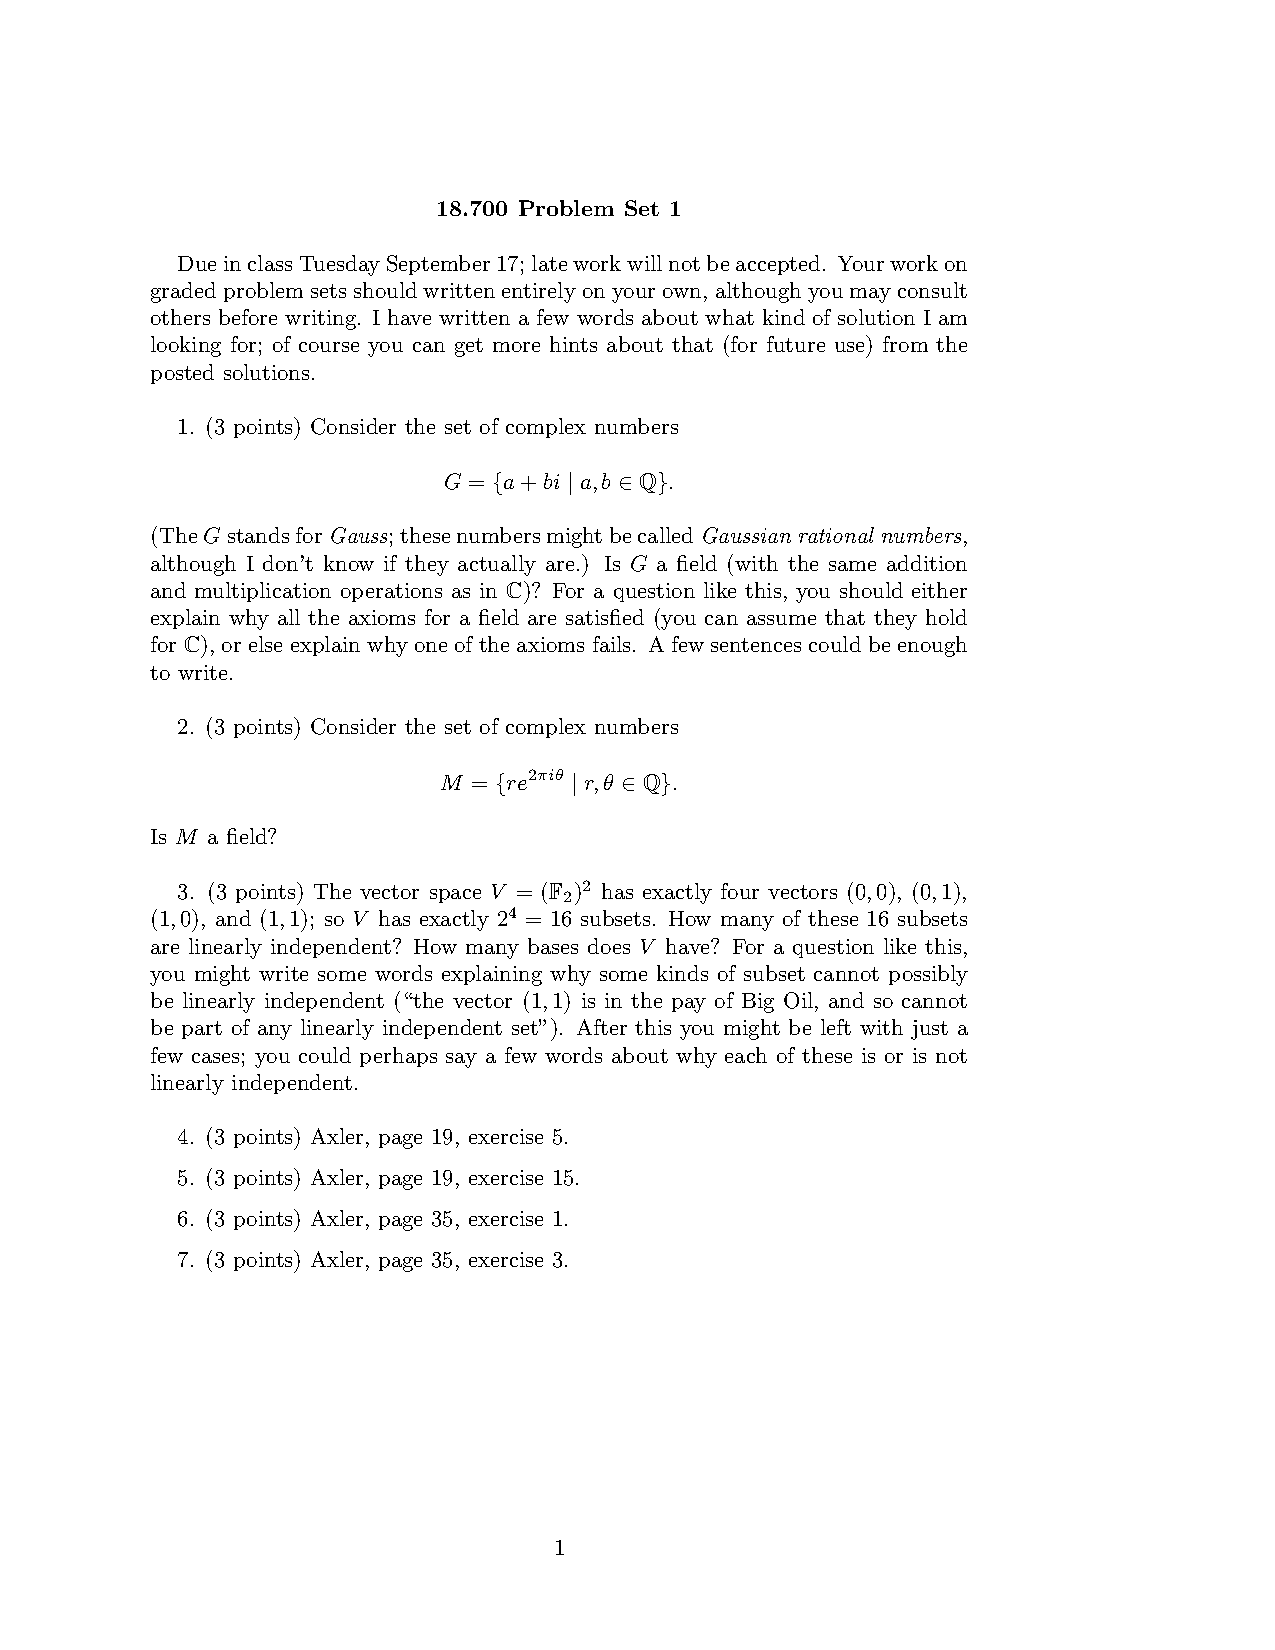
\includepdf[link=true, linkname=LinearAlgebra-ProblemSet1,pages=1]{MIT/Problems/18.700/ProblemSet1.pdf}
\section*{Question 1}
Instead of proving $ G $ is a field directly, it is easier to observe that $ G $ is a subset of $ C $, and so we can prove that $ G $ is a field by proving this lemma first:

If $ H $ is a subset of a field $ F $, then $ H $ is a field (inheriting the operations from $ F $) if 
\begin{enumerate}
    \item There exists an element $ h \ne 0 \in H $, 
    \item for all $ p, q \in H $, $ p - q \in H $, and
    \item for all $ p, q \ne 0 \in H $, $ \frac{p}{q} \in H $.
\end{enumerate}

By setting $ p = q = h $, using the rule 2 and 3, we get that $ 0 \in H $ and $ 1 \in H $. By setting $ p = 0 $, using rule 2, we get that additive inverse exists in $ H $. By setting $ p = 1 $, using rule 3, we get that multiplicative inverse exists in $ H $. Using inverses, we know sum and product exists in $ H $. All other field axioms simply inherits from $ F $, therefore $ H $ is a field.

With the lemma, in order to prove that $ G $ is a field. It suffice to show the three conditions. 

\begin{enumerate}
    \item we have  $ 1 + 0i \in H $, 
    \item for any $ (a + bi), (c + di) \in G $, we have $ (a + bi) - (c + di) = (a-c) + (b-d)i \in G $. 
    \item for any $ (a + bi), (c + di) \in G $, we have $ \frac{a + bi}{c + di} = \frac{(a+bi)(c-di)}{c^2 + d^2} = \frac{ac+bd}{c^2+d^2} + \frac{bc-ad}{c^2+d^2}i \in G $.
\end{enumerate}

Therefore we conclude $ G $ is a field.
\section*{Question 2}
$ M $ is not a field because $ e^{2 \pi i \left(\frac{1}{4}\right)} + e^{2 \pi i (0)} = i + 1 = \sqrt{2} e^{2 \pi i \frac{1}{8} i} \notin M $
\section*{Question 3}
To start with, $ (0, 0) $ cannot be part of a basis, so we are left with 3 vectors.

Obviously, $ \{(1, 0), (0, 1)\} $ is a basis, so we know the dimension of the vector space is 2.

All $ \left( \begin{array}{c} 3 \\ 2 \end{array} \right) $ subsets of vector is a basis, because of the following:

\begin{eqnarray*}
\left|
\begin{array}{cc}
  1 & 0 \\
  0 & 1
\end{array}
\right| &=& 1 \\
\left|
\begin{array}{cc}
  1 & 1 \\
  0 & 1
\end{array}
\right| &=& 1 \\
\left|
\begin{array}{cc}
  0 & 1 \\
  1 & 1
\end{array}
\right| &=& 1
\end{eqnarray*}
As a reminder, if the determinant is non-zero, that means an inverse exists. That inverse can be used to construct linear combinations of the vectors so that they construct the standard basis. That's why the vectors span the whole space.
\section*{Question 4}
Note that $ F^3 $ stands for either $ R^3 $ or $ C^3 $ in the book.
\subsection*{Part a}
It is a vector space because:
\begin{enumerate}
    \item {$ (0, 0, 0) $ is in the subset}
    \item { If $ a + 2b + 3c = 0 $ and $ d + 2e + 3f = 0 $, then $ (a + d) + 2(b + e) + 3 (c + f) = 0 $. Therefore, whenever $ (a,b,c) $ and $ (d,e,f) $ belongs to the subset, then $ (a,b,c) + (d,e,f) = ((a+d),(b+e),(c+f)) $ belongs to the subset too, which means the space is closed under addition.}
    \item { If $ a + 2b + 3c = 0 $ then $ (fa) + 2(fb) + 3(fc) = 0 $. Therefore, whenever $ (a,b,c) $ belongs to the subset, then $ f(a, b, c) = (fa, fb, fc) $ belongs to the subset too, which means the space is closed under scalar multiplication.}
\end{enumerate}

\subsection*{Part b}
The vector $ (0, 0, 0) $ does not belong to the subset and therefore it is not a subspace.

\subsection*{Part c}
The vector $ (1, 1, 0) $ and $ (0, 0, 1) $ belongs to the subset but their sum $ (1, 1, 1) $ is not, therefore it is not a subspace.

\subsection*{Part d}
It is a vector space because:
\begin{enumerate}
    \item {$ (0, 0, 0) $ is in the subset}
    \item { If $ a = 5c $ and $ d = 5f $, then $ (a + d) = 5(c + f) $. Therefore, whenever $ (a,b,c) $ and $ (d,e,f) $ belongs to the subset, then $ (a,b,c) + (d,e,f) = ((a+d),(b+e),(c+f)) $ belongs to the subset too, which means the space is closed under addition.}
    \item { If $ a = 5c $ then $ (fa) = 5(fc) $. Therefore, whenever $ (a,b,c) $ belongs to the subset, then $ f(a, b, c) = (fa, fb, fc) $ belongs to the subset too, which means the space is closed under scalar multiplication.}
\end{enumerate}

Apparently, this proof is the same as part a. In fact, it follows that a set of vectors satisfying a system of homogeneous linear equations (i.e. with 0 constant terms) is a subspace, and the proof is going to be identical. 
\section*{Question 5}
I have spent some time (an hour maybe) trying to prove that $ U_1 = U_2 $, but turn out that is wasted effort because $ U_1 \ne U_2 $.

As a counter example, consider:
\begin{enumerate}
  \item {$ U_1 $ to be the vector space spanned by the vectors $ \{ (1, 0) \} $.}
  \item {$ U_2 $ to be the vector space spanned by the vectors $ \{ (1, 1) \} $.}
  \item {$ W $ to be the vector space spanned by the vectors $ \{ (0, 1) \} $.}
  \item {$ V $ to be $ F^2 $.}
\end{enumerate}
\section*{Question 6}
To prove that the new set of vectors spans all the vectors spanned by the old set. One must prove that for all vectors spanned in the old set, it can be spanned by the new set. Solving that problem directly is difficult, let's us consider in general what can the new set of vector span by considering the general linear combination of the new set as follows:

\begin{eqnarray*}
  & & d_1 (v_1 - v_2) + d_2 (v_2 - v_3) + \cdots + d_{n-1}(v_{n-1} - v_n) + d_n v_n \\
  &=& d_1 v_1 - d_ 1 v_2 + d_2 v_2 - d_2 v_3 + \cdots + d_{n-1} v_{n-1} - d_{n-1} v_n + d_n v_n \\
  &=& d_1 v_1 + (d_2 - d_1) v_2 + (d_3 - d_2) v_3 + \cdots + (d_n - d_{n-1}) v_n \\
  &=& c_1 v_1 + c_2 v_2 + \cdots + c_n v_n
\end{eqnarray*}

If we read it backwards, the idea is that if we could find $ d_i $ in terms of $ c_i $, then we solved the problem. It is obvious that $ d_1 = c_1 $, and also, for all $i \ge 2 $, $ d_i - d_{i-1} = c_i $. A simple manipulation yield the recurrence relation $ d_i = d_{i-1} + c_i $, which gives $ d_i = \sum\limits_{k=1}^{i}{c_k} $. That solved our problem!

To present this formally, we prove that 
\begin{eqnarray*}
  & & d_1 (v_1 - v_2) + d_2 (v_2 - v_3) + \cdots + d_{n-1}(v_{n-1} - v_n) + d_n v_n \\
  &=& \sum\limits_{i=1}^{n-1} d_i (v_i - v_{i+1}) + d_n v_n \\
  &=& \sum\limits_{i=1}^{n-1} d_i v_i - \sum\limits_{i=1}^{n-1} d_i v_{i+1} + d_n v_n \\
  &=& \sum\limits_{i=1}^{n-1} \sum\limits_{k=1}^{i}{c_k} v_i - \sum\limits_{i=1}^{n-1} \sum\limits_{k=1}^{i}{c_k} v_{i+1} + \sum\limits_{k=1}^{n}{c_k} v_n \\
  &=& \sum\limits_{i=1}^{n-1} \sum\limits_{k=1}^{i}{c_k} v_i - \sum\limits_{i=2}^{n} \sum\limits_{k=1}^{i-1}{c_k} v_{i} + \sum\limits_{k=1}^{n}{c_k} v_n \\
  &=& c_1 v_1 + \sum\limits_{i=2}^{n-1} \sum\limits_{k=1}^{i}{c_k} v_i - \sum\limits_{i=2}^{n} \sum\limits_{k=1}^{i-1}{c_k} v_{i} + \sum\limits_{k=1}^{n}{c_k} v_n \\
  &=& c_1 v_1 + \sum\limits_{i=2}^{n-1} \left(\sum\limits_{k=1}^{i-1}{c_k} v_i + c_iv_i\right) - \sum\limits_{i=2}^{n} \sum\limits_{k=1}^{i-1}{c_k} v_{i} + \sum\limits_{k=1}^{n}{c_k} v_n \\
  &=& c_1 v_1 + \sum\limits_{i=2}^{n-1} \sum\limits_{k=1}^{i-1}{c_k} v_i + \sum\limits_{i=2}^{n-1} c_iv_i - \sum\limits_{i=2}^{n} \sum\limits_{k=1}^{i-1}{c_k} v_{i} + \sum\limits_{k=1}^{n}{c_k} v_n \\
  &=& c_1 v_1 + \sum\limits_{i=2}^{n-1} \sum\limits_{k=1}^{i-1}{c_k} v_i + \sum\limits_{i=2}^{n-1} c_iv_i - \sum\limits_{i=2}^{n-1} \sum\limits_{k=1}^{i-1}{c_k} v_{i} - \sum\limits_{k=1}^{n-1}{c_k} v_n + \sum\limits_{k=1}^{n}{c_k} v_n \\
  &=& c_1 v_1 + \sum\limits_{i=2}^{n-1} c_iv_i - \sum\limits_{k=1}^{n-1}{c_k} v_n + \sum\limits_{k=1}^{n}{c_k} v_n \\
  &=& c_1 v_1 + \sum\limits_{i=2}^{n-1} c_iv_i + c_n v_n \\
  &=& c_1 v_1 + c_2 v_2 + \cdots + c_n v_n
\end{eqnarray*}

The manipulation is tedious and obscure the original idea, that's why I wrote the above before the formal presentation. The key trick is to arrange the two big double summations introduced in line 4 to cancel each other. Most steps after line 4 is just to make sure all the indices matches up so that we can cancel. We knew that's the answer, so any terms that left will form exactly the linear combination we need.
\section*{Question 7}
Since $ \{v_1 + w, v_2 + w, \cdots v_n + w \}$ is linearly dependent, there exists $ c_i $ not all zero such that $ \sum\limits_{i=1}^{n} c_i(v_i + w) = 0 $. A simple manipulation shows that $ \left(\sum\limits_{i=1}^{n} c_i \right) w = \sum\limits_{i=1}^{n} -c_i v_i $.

Suppose (for the sake of contradiction) that $ D = \sum\limits_{i=1}^{n} c_i = 0 $, then the left hand side of the equation is 0 and we have found a non-trivial linear combination of $ v_i $ that sums to zero, contradicting the fact the $ \{v_1, v_2, \cdots, v_n \} $ is linearly independent. Therefore $ D \ne 0 $, and $ w = \sum\limits_{i=1}^{n} -\frac{c_i}{D} v_i $ so $ w \in span(\{v_1, v_2, \cdots, v_n \}) $.

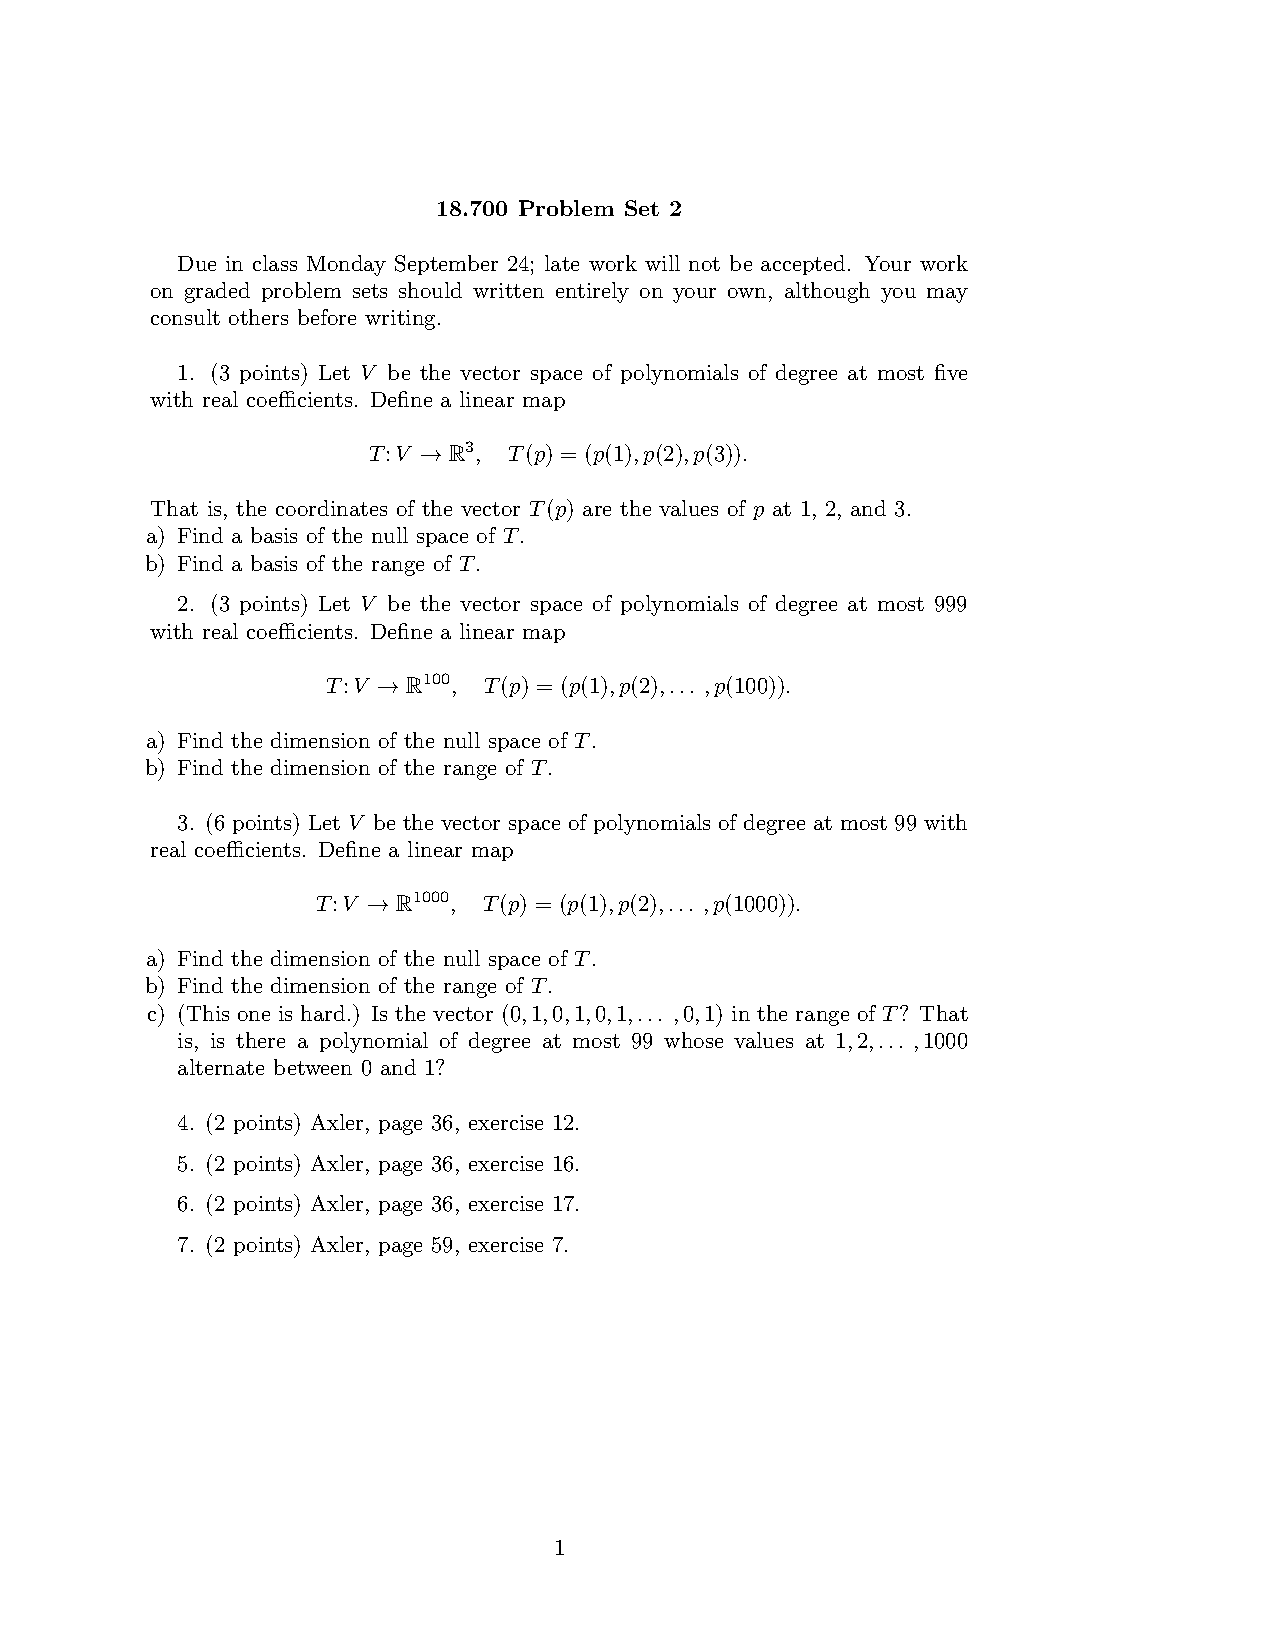
\includepdf[link=true, linkname=LinearAlgebra-ProblemSet2,pages=1]{MIT/Problems/18.700/ProblemSet2.pdf}
\section*{Question 1}
\subsection*{Part a}
The null space $ ker(T) $ of the linear transformation $ T $ is precisely the set of polynomials $ f $ of degree at most 5, such that $ f(1) = f(2) = f(3) = 0 $. Obviously, all such polynomial must have a factor of $ (x - 1)(x - 2)(x - 3) $. 

To simplify, let's consider the mapping $ M : ker(T) \mapsto U, M(p) = \frac{p}{(x - 1)(x - 2)(x - 3)} $

Denote $ U' $ to be the set of all polynomials with real coefficients of degree at most 2.

$ U \subset U' $ because any polynomial in $ ker(T) $ must have a factor of $ (x - 1)(x - 2)(x - 3) $ and of degree at most 5, so $ M(p) $ must be a polynomial with real coefficients with degree at most 2.

$ U' \subset U $ because when $ q \in U' $, $ f = q(x - 1)(x - 2)(x - 3) $ is a polynomial with real coefficients with degree at most 5 and $ f(1) = f(2) = f(3) = 0 $, that implies $ f \in ker(T) $ and so $ q \in U $

So $ U = U' $, but not only that, it is a vector space isomorphism because the mapping is bijective and it respects the add and scalar multiply operations.

$ U' $ has a very simple basis of $ B' = \{1, x, x^2 \} $, therefore, a basis of $ ker(T) $ is $ B = M^{-1}(B') = \{(x - 1)(x - 2)(x - 3), x(x - 1)(x - 2)(x - 3), x^2(x - 1)(x - 2)(x - 3) \} $.

\subsection*{Part b}
Using Lagrange's interpolation, for any $ (a,b,c) \in R^3 $, we can create polynomials in real coefficients that satisfy $ p(1) = a, p(2) = b, p(3) = c $ as follows:

$ \frac{(x-2)(x-3)}{(1-2)(1-3)}a + \frac{(x-1)(x-3)}{(2-2)(2-3)}b + \frac{(x-1)(x-2)}{(3-1)(3-2)}c $

That means $ Im(T) = R^3 $, which means we have a very simple basis for $ Im(T) = \{(1,0,0), (0,1,0), (0,0,1) \} $.
\section*{Question 2}
\subsection*{Part a}
Using the same trick as in question 1, $ ker(T) $ is isomorphic to the space of polynomials with real coefficients of degree at most $ 899 $, therefore the dimension of $ ker(T) $ is 899. 

\subsection*{Part b}

Using the same trick as in question 1, $ Im(T) $ is isomorphic to $ R^{100} $, therefore the dimension of $ Im(T) $ is 100.
\section*{Question 3}
\subsection*{Part a}
The only polynomial of degree at most 99 having 1000 zeros is $ f(x) = 0 $. Therefore the dimension of $ Ker(T) $ is 0.
\subsection*{Part b}
By the rank nullity theorem, $ dim(Ker(T)) + dim(Im(T)) = dim(V) $ where $ V $ is the domain of the linear transformation $ T $. Therefore the dimension of $ Im(T) $ is 100.
\subsection*{Part c}
The only polynomial of degree at most 99 having 500 zeros is $ f(x) = 0 $. But then $ f(2) = 0 \ne 1 $, therefore such a polynomial does not exist and $ (0,1,\cdots,0,1) \notin Im(T) $.
\section*{Question 4}
Since $ p_j(2) = 0 $, $ (x-2) $ is a factor of $ p_j $ for all $ j $. Consider the polynomials $ q_j = \frac{p_j}{x-2} $. These are $ m + 1 $ polynomials of degree at most $ m - 1 $, these must be linearly dependent because $ dim(p_{m-1}) = m $. So there exists a non-trivial linear combination $ \sum\limits_{i=0}^{m} c_i q_i = 0 $. Multiply by $ (x - 2) $, we have got a non-trivial linear combination $ \sum\limits_{i=0}^{m} c_i p_i = 0 $ so that these vectors are not linearly independent.
\section*{Question 5}
Since $ U_1, U_2 \cdots U_m $ are vector spaces, there exists $ B_1, B_2 \cdots B_n $ bases for them. Any vectors in $ U_1 + U_2 + \cdots + U_n $ can be written a a sum of vectors $ u_1 + u_2 + \cdots + u_n $, which can in turn written into the sum of linear combination of these basis vectors. That means $ B_1 \cup B_2 \cup \cdots \cup B_n $ spans $ U_1 + U_2 + \cdots + U_n $. The dimension is always at most the size of a spanning set, so:

\begin{eqnarray*}
    &   & dim(U_1 + U_2 + \cdots + U_n) \\
    &\le& | B_1 \cup B_2 \cup \cdots \cup B_n | \\
    &\le& | B_1 | + | B_2 | + \cdots + | B_n | \\
    &=  & dim(U_1) + dim(U_2) + \cdots + dim(U_n)
  \end{eqnarray*}
\section*{Question 6}
Using the same idea as in question 5, except we claim that the generated spanning set is actually a basis.

Suppose (for the sake of contradiction) that the spanning set is not linearly independent, then there exists a non-trivial linear combination. 

\begin{eqnarray*}
    w_1 b_1 + w_2 b_2 + \cdots w_k b_k = 0
\end{eqnarray*}

Furthermore, we can enforce some more conditions. First, $ w_j \ne 0 $ for all $ j $, this can be easily done by dropping the zero terms. Second, this sum must involve basis vectors coming from more than one vector space. This must be true because otherwise we contradict the fact that the vectors selected is a basis.

Without loss of generality, we assume $ U_1 $ is involved in the sum, and we split the sum as follow:

\begin{eqnarray*}
    (w_{11} p_1 + w_{12} p_2 + \cdots w_{1k_1} p_{k_1}) + (w_{21} q_1 + w_{22} q_2 + \cdots w_{k_2} q_{k_2}) = 0
\end{eqnarray*}

Where $ p_j $ comes from $ U_1 $ and $ q_j $ does not come from $ U_1 $.

Now it is clear that the first part of the sum is simply a vector (which we will call $ p $) in $ U_1 $, and we have found a linear combination of it by combining vectors in some other vector spaces.

Now we have found our contradiction. $ p $ can be represented as either $ p $ or the linear combination we have just found, contradicting the fact that the combined vector space is a direct sum, which requires all vectors in it have a unique representation as a sum of individual vector spaces.
\section*{Question 7}
As $ T $ is surjective, for any vector $ t $ in $ V $, there exists a vector $ v \in V $ such that $ T(v) = t $. Now $ v $ can be represented as a linear combination of the basis vector of $ V $ and $ T $ is linear, so we can apply $ T $ to both sides and so $ T(v_1) T(v_2) \cdots T(v_n) $ span $ W $.

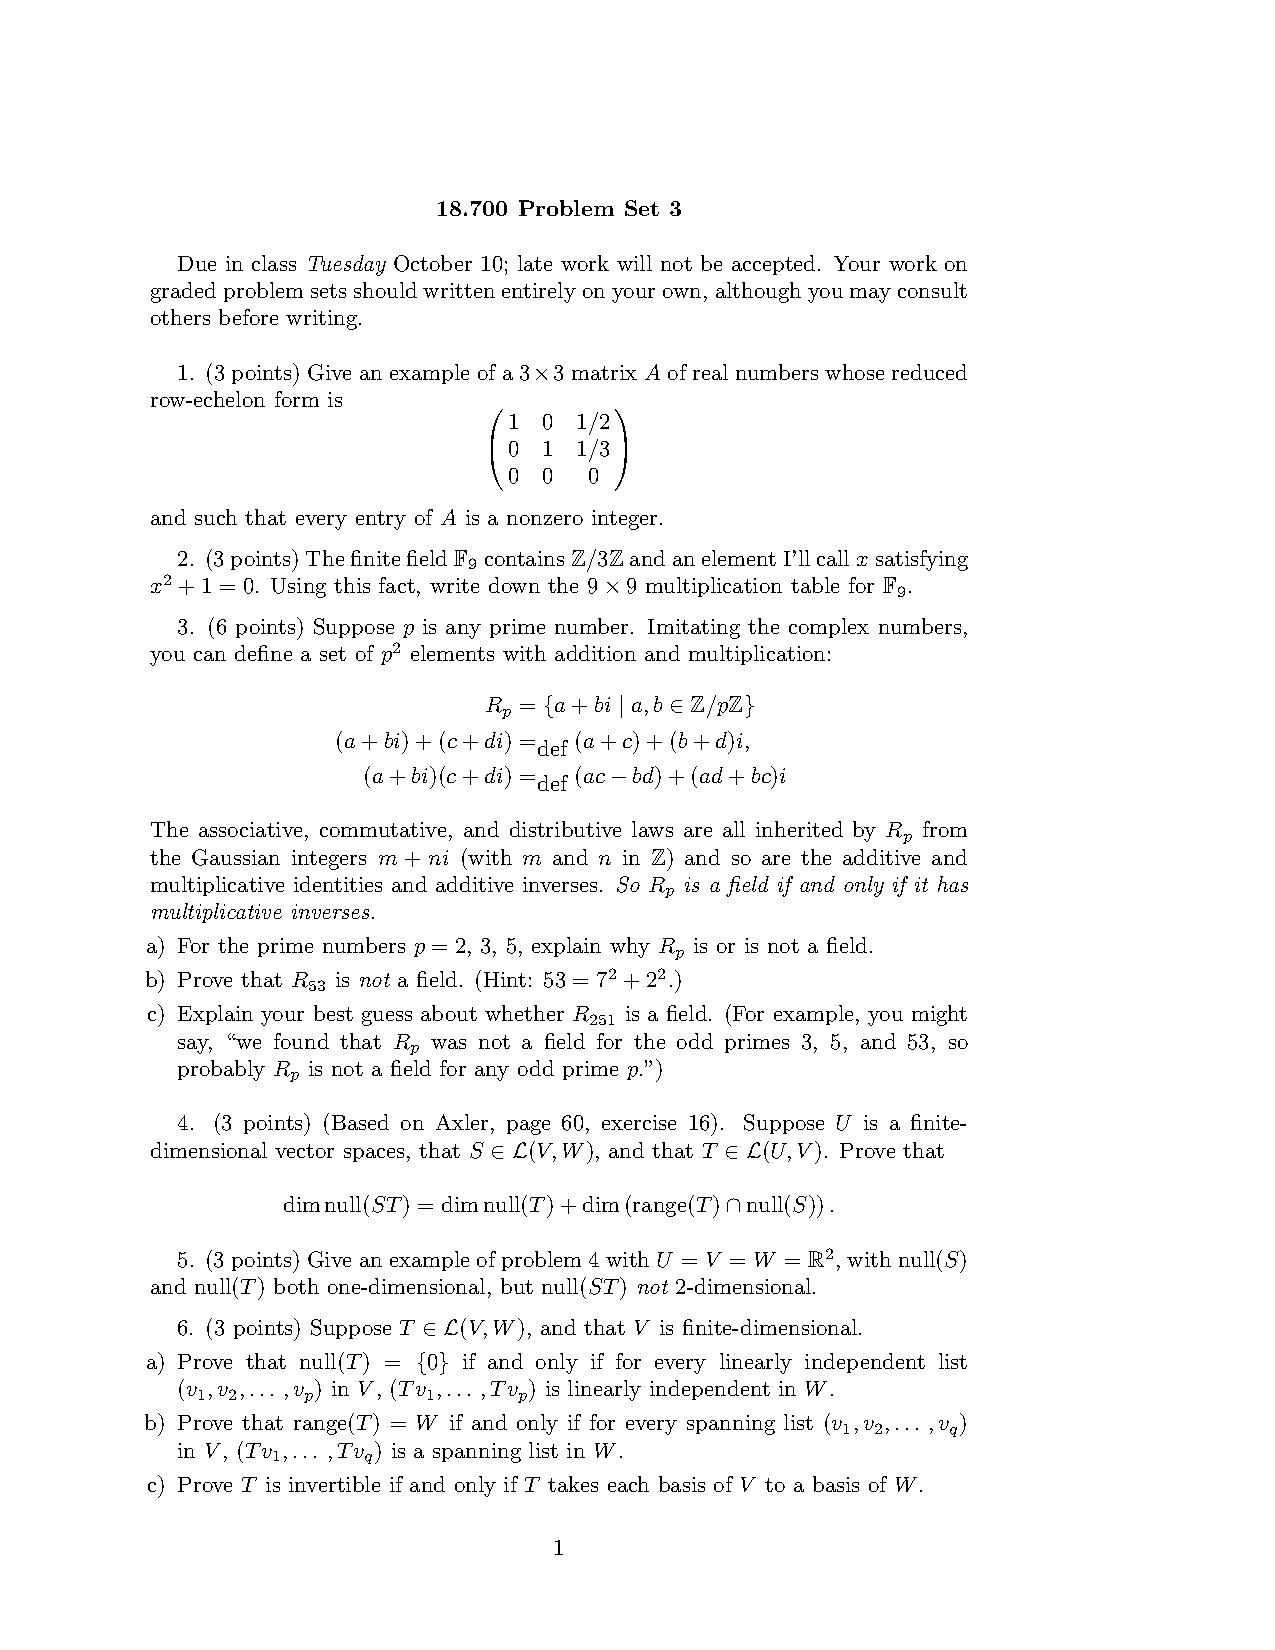
\includepdf[link=true, linkname=LinearAlgebra-ProblemSet3,pages=1]{MIT/Problems/18.700/ProblemSet3.pdf}
\section*{Question 1}
\begin{eqnarray*}
  & & \left(
        \begin{array}{ccc}
          1 & 0 & \frac{1}{2} \\
          0 & 1 & \frac{1}{3} \\
          0 & 0 & 0 
        \end{array}
      \right) \\
  & \to &
    \left(
        \begin{array}{ccc}
          2 & 0 & 1 \\
          0 & 3 & 1 \\
          0 & 0 & 0 
        \end{array}
    \right) \\
  & \to &
    \left(
        \begin{array}{ccc}
          2 & 3 & 2 \\
          0 & 3 & 1 \\
          0 & 0 & 0 
        \end{array}
    \right) \\
  & \to &
    \left(
        \begin{array}{ccc}
          2 & 3 & 2 \\
          2 & 6 & 3 \\
          0 & 0 & 0 
        \end{array}
    \right) \\       
  & \to &
    \left(
        \begin{array}{ccc}
          2 & 3 & 2 \\
          2 & 6 & 3 \\
          2 & 6 & 3
        \end{array}
    \right) \\           
\end{eqnarray*}

\section*{Question 2}
The key idea is that the $ F_9 $ elements are $ 0, 1, 2, x, x + 1, x + 2, 2x, 2x + 1 $ and $ 2x + 2$. Once we have that, the rest is simply doing all the 9 x 9 multiplication. Here are the results:
\begin{eqnarray*}
  & & \left(
        \begin{array}{ccccccccc}
0 & 0 & 0 & 0 & 0 & 0 & 0 & 0 & 0 \\
0 & 1 & 2 & x & x + 1 & x + 2 & 2x & 2x + 1 & 2x + 2 \\
0 & 2 & 1 & 2x & 2x + 2 & 2x + 1 & x & x + 2 & x + 1 \\
0 & x & 2x & 2 & x + 2 & 2x + 2 & 1 & x + 1 & 2x + 1 \\
0 & x + 1 & 2x + 2 & x + 2 & 2x & 1 & 2x + 1 & 2 & x \\
0 & x + 2 & 2x + 1 & 2x + 2 & 1 & x & x + 1 & 2x & 2 \\
0 & 2x & x & 1 & 2x + 1 & x + 1 & 2 & 2x + 2 & x + 2 \\
0 & 2x + 1 & x + 2 & x + 1 & 2 & 2x & 2x + 2 & x & 1 \\
0 & 2x + 2 & x + 1 & 2x + 1 & x & 2 & x + 2 & 1 & 2x \\
        \end{array}
      \right) \\
\end{eqnarray*}

Of course, I am not going to do that 81 multiplications myself, the work is done by these simple python code:

\begin{verbatim}
e = []

def mul(x,y):
    (a,b) = x
    (c,d) = y
    # (ax + b)(cx + d)
    # = acx^2 + (ad + bc)x + bd
    # = (ad + bc)x + (bd - ac)
    p = (a * d + b * c) % 3
    q = (b * d - a * c + 3) % 3
    if (p == 0):
        return q
    elif p == 1:
        if q == 0:
            return "x"
        else:
            return "x + %s" % q
    else:
        if q == 0:
            return "2x"
        else:
            return "2x + %s" % q

for c in range(0, 3):
    for d in range(0, 3):
        e.append((c,d))

for p in e:
    for q in e:
        print(mul(p,q),end=" ")
    print()

\end{verbatim}
\section*{Question 3}
Consider the multiplicative inverse of a general element of $ (a + bi) $ 

\begin{eqnarray*}
  & & \frac{1}{a + bi} \\
  &=& \frac{a - bi}{a^2 + b^2} \\
\end{eqnarray*}

Now since $ a, b \in Z/pZ $ which is a field, so as long as $ a^2 + b^2 \ne 0 $, the multiplicative inverse of $ a^2 + b^2 $ exists and therefore the multiplicative inverse of $ a^2 + b^2 $ exists.

To be continued
\section*{Question 4}
First, $ null(T) $ is a vector space and therefore has a basis $ t_1, t_2, ..., t_m \in U $. Also, $ null(S) $ and $ range(T) $ are vector spaces, so $ null(S) \cap range(T) $ is also a vector space and therefore has a basis $ v_1, v_2, \cdots v_n $. Each of these $ n $ vectors must have a preimage $ u_1, u_2, \cdots u_n \in U $ such that $ T(u_i) = v_i $. I claim that $ B = \{ t_1, t_2, ..., t_m, u_1, u_2, \cdots u_n \} $ is a basis for $ null(ST) $.

To show that the $ B $ spans $ null(ST) $, consider a general vector $ v \in null(ST) $. $ T(v) \in null(S) \cap range(T) $, so it can be written as a unique linear combination $ T(v) = \sum c_i v_i $. Consider: 

\begin{eqnarray*}
  & & T(v - \sum c_i u_i) \\
  &=& T(v) - \sum c_i T(u_i) \\
  &=& T(v) - \sum c_i v_i \\
  &=& T(v) - T(v) \\
  &=& 0 
\end{eqnarray*}

That means $ (v - \sum c_i u_i) \in null(T) $ and therefore:

\begin{eqnarray*}
  v - \sum c_i u_i &=& \sum d_i t_i \\
                 v &=& \sum c_i u_i + \sum d_i t_i 
\end{eqnarray*}

So $ B $ spans $ null(ST) $.

To show that $ B $ is linearly independent, suppose (for the sake of contradiction) there exists a non-trivial linear combination $ \sum c_i u_i + \sum d_i t_i = 0 $. Suppose $ c_i = 0 $ for all $ i $, we have a non-trivial linear combination $ \sum d_i t_i = 0 $, contradicting the fact that $ t_i $ is a basis of $ null(T) $. Therefore, there must be an $ c_i \ne 0 $. Applying $ T $ on the linear combination, we get 

\begin{eqnarray*}
     \sum c_i u_i + \sum d_i t_i &=& 0 \\
  T(\sum c_i u_i + \sum d_i t_i) &=& T(0) \\
  \sum c_i T(u_i) + \sum d_i T(t_i) &=& 0 \\
  \sum c_i v_i &=& 0 
\end{eqnarray*}

Now we have found a non-trivial linear combination of 0 of $ v_i $, that contradicts the fact that $ v_i $ is a basis of $ null(S) \cap range(T) $. Therefore $ B $ must be linearly independent.

$ B $ spans $ null(ST) $ and is linearly independent, therefore $ B $ is a basis of $ null(ST) $ and $ dim(null(ST)) = m + n = dim(null(T)) + dim (null(S) \cap range(T)) $.
\section*{Question 5}
It is given that $ dim(null(S)) = dim(null(T)) = 1 $, so the only way for $ dim(null(ST)) < 2 $ is when $ dim(range(T) \cap null(S)) = 0 $. By rank nullity theorem, we know $ dim(range(T)) = 1 $. Therefore it makes sense to construct $ S $ and $ T $ such that $ range(T) $ and $ null(S) $ are both one dimensional subspace and yet only intersect at 0.

The easiest one dimensional subspaces are the x and y axis. Let's decide that $ range(T) $ is the x-axis and $ null(S) $ is the y-axis. To satisfy these constraints, we can set

\begin{eqnarray*}
  S((x,y)) &=& (x,0) \\
  T((x,y)) &=& (x,0)
\end{eqnarray*}

We can easy check that $ ST((x,y)) = (x,0) $ and therefore $ dim(null(ST)) = 1 $ as required.
\section*{Question 6}
\subsection*{Part a}
To prove $ \implies $, we have $ null(T) = \{0\} $ and assume $ T(v_1), \cdots  , T(v_p) $ is linearly dependent, there exists non-trivial $ c_i $ such that $ \sum c_i T(v_i) = 0 $. Simplifying, we get $ T(\sum c_i v_i) = T(0) = 0 $, but $ \sum c_i v_i \ne 0 $ because $ c_i $ is non-trivial and $ v_i $ are linearly independent, that contradicts $ null(T) = \{0\} $. This proves $ \implies $.

To prove $ \impliedby $, assume $ v \ne 0 $ and $ T(v) = 0 $.  $ v $ can be written as $ \sum c_i v_i $ for a basis $ v_i $ of $ v $. Since $ v \ne 0 $, some of the $ c_i $ must be non zero. Now $ 0 = T(v) = T(\sum c_i v_i) = \sum c_i T(v_i) $. This is a non-trivial (since there exists a $ c_i \ne 0 $) linear combination of a list of linear independent vector to 0. That is a contradiction. This proves $ \impliedby $.

\subsection*{Part b}
To prove $ \implies $, we have $ range(T) = W $ and assume there exists a spanning list of $ V = \{v_1, \cdots v_p\}$, $ T(v_1), \cdots , T(v_p) $ is does not span $ W $. For any vector $ w \in W $, there exists a $ v \in V $ such that $ T(v) = w $, now $ v $ can be written as $ \sum c_i v_i $. By applying $ T $, we get $ w = T(v) = T(\sum c_i v_i) = \sum c_i T(v_i) $. Now we have show that any vector can be written as a linear combination of $ T(v_i) $ contradicting the assumption $ T(v_1), \cdots , T(v_p) $ is does not span $ W $. This proves $ \implies $.

To prove $ \impliedby $, assume there exists $ w \in W \notin range(T) $. For a basis $ v_1, \cdots , v_n $, $ T(v_1), \cdots , T(v_n) $ span $ W $, so $ w $ can be written as $ w = \sum(c_i T(v_i)) $, but then $ T(\sum c_i v_i) = w $ and so $ w \in range(T) $. This contradiction proves $ \impliedby $.

\subsection*{Part c}
First, we prove this lemma that $ T$ is injective if and only if $ null(T) = \{0\} $.

To prove $ \implies $. $ T $ is injective, so if $ T(x) = 0 $, we also have $ T(0) = 0 $, so $ T(x) = T(0) $, by the injectivity of $ T $, $ x = 0 $, so $ null(T) = \{0\} $.

To prove $ \impliedby $. If $ T(x) = T(y) $, then $ T(x - y) = T(0) = 0 $, $ null(T) = \{0\} $ implies $ x - y = 0 $, and so $ x = y $ and we proved the injectivity of $ T $.

Combining part a, part b and this lemma give us the proof:

\begin{enumerate}
    \item $ T $ is invertible.
    \item if and only if $ T $ is injective and sujective.
    \item if and only if $ null(T) = \{0\} $ and $ range(T) = W $
    \item if and only if T takes linearly independent list to linearly independent list and T takes spanning set to spanning set.
    \item if and only if T takes basis to basis.
\end{enumerate}

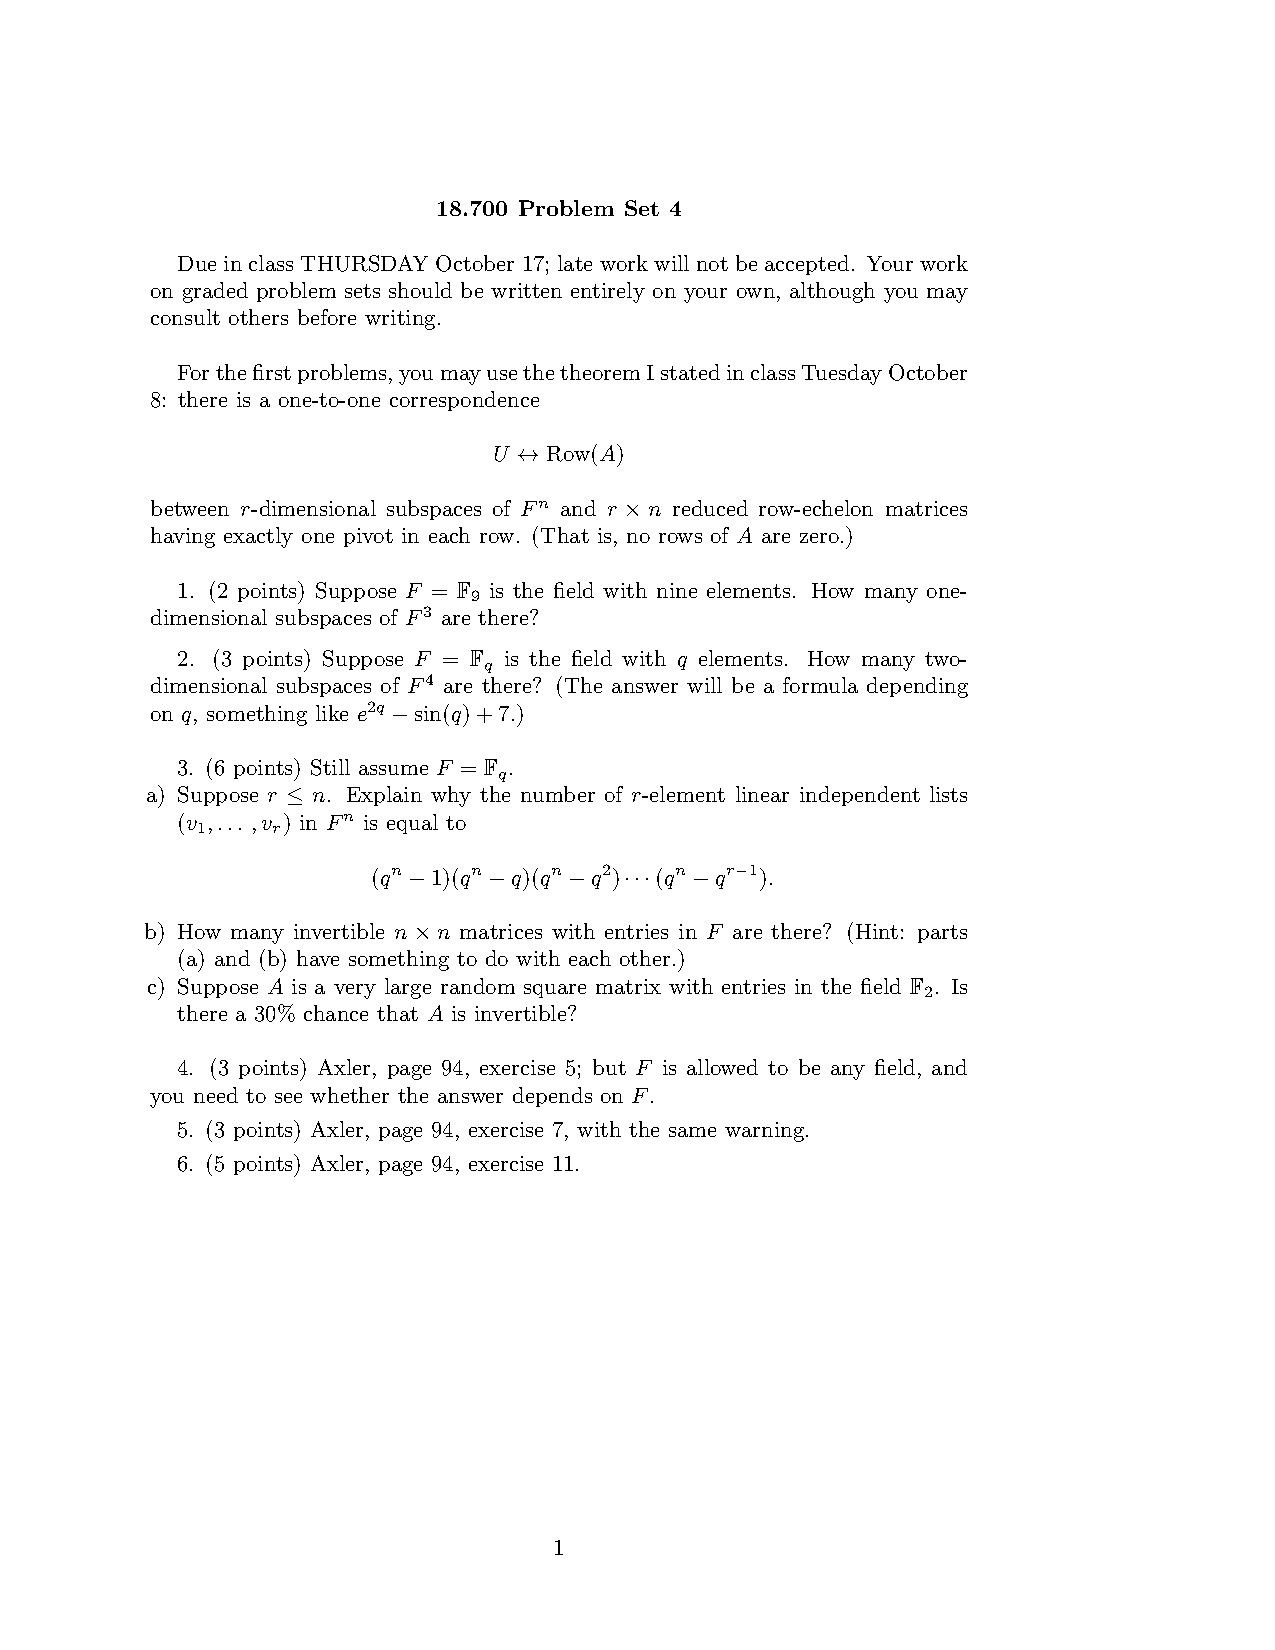
\includepdf[link=true, linkname=LinearAlgebra-ProblemSet4,pages=1]{MIT/Problems/18.700/ProblemSet4.pdf}
\section*{Question 1}
Since the subspaces are one to one mapped with the matrices in the row reduced echelon form, it is much easier to count those matrices.

The row reduced echelon form can be in one of the following 3 cases:

\begin{eqnarray*}
  \left(1, x, y\right)
  \left(0, 1, x\right)
  \left(0, 0, 1\right)
\end{eqnarray*}

There are $ 9 \times 9 = 81 $ different matrices of the first form. $ 9 $ matrices of the second form and 1 matrix of the last form. There are $ 81 + 9 + 1 = 91 $ different row educed echelon matrices, and therefore there are 91 different subspace of 1 dimension.

To verify this is the right solution, I started learning \href{https://www.sagemath.org/}{Sage}. Here is some sage code that verify that there is indeed 91 subspaces. The code simply iterate through all possible vectors in $ F^3 $ and then canonicalize them using the echelon form and count how many distinct subspaces there are. Obviously, we must discount the $ \left(0, 0, 0\right) $ special case for safety sake.

\begin{verbatim}
Field = GF(9)
MatrixOnField = MatrixSpace(Field,1,3)
elements = []
for _,element in enumerate(Field):
  elements.append(element)
Subspaces = {}
for p in elements:
  for q in elements:
    for r in elements:
      Reduced = MatrixOnField([p,q,r]).echelon_form()
      if Reduced[0] != MatrixOnField([0,0,0])[0]:
        Subspaces[Reduced] = True
len(Subspaces)
\end{verbatim}
\section*{Question 2}
Using the same idea as in question 1, the row reduced echelon form can be in one of the following cases:

\begin{eqnarray*}
  \left(
  \begin{array}{cccc}
  1, 0, a, b \\
  0, 1, c, d
  \end{array}
  \right) \\
  \left(
  \begin{array}{cccc}
  1, a, 0, b \\
  0, 0, 1, c
  \end{array}
  \right) \\
  \left(
  \begin{array}{cccc}
  1, a, b, 0 \\
  0, 0, 0, 1
  \end{array}
  \right) \\
  \left(
  \begin{array}{cccc}
  0, 1, 0, a \\
  0, 0, 1, b
  \end{array}
  \right) \\
  \left(
  \begin{array}{cccc}
  0, 1, a, 0 \\
  0, 0, 0, 1
  \end{array}
  \right) \\
  \left(
  \begin{array}{cccc}
  0, 0, 1, 0 \\
  0, 0, 0, 1
  \end{array}
  \right)
\end{eqnarray*}
Using these cases, we will have $ q^4 + q^3 + 2q^2 + q + 1 $ row reduced echelon matrices, and therefore having the same number of vector subspaces of dimension 2.
\section*{Question 3}
\subsection*{Part a}
In $ F^n $, there are $ q^n $ vectors. One of them is the zero vector that we must exclude. Otherwise, all $ q^n - 1 $ vector could be the first vector in the list. That's why we have the $ (q^n - 1) $ as the first factor.

For each vector $ v $ as the first vector, $ \{ v, 2v, \cdots (q-1)v \} $ is a set of $ q - 1 $ vectors that should also be excluded as the second vector. That gives us the second factor of $ (q^n - 1) - (q - 1) = (q^n - q) $.

For each pair of vector $ v $ and $ w $ as the first two vectors, $ \{ v, v + w, \cdots, v + (q-1)w, 2v, 2v + w, \cdots 2v + (q-1)w, \cdots (q-1)v + (q-1)w \} $ is a set of $ (q^2 - 1) $ vectors that should be excluded as the third vector. That gives us the third factor of $ (q^n - 1) - (q^2 - 1) = (q^n - q^2) $.

The argument goes on and eventually lead to the expression we wanted.

\subsection*{Part b}
An $ n \times n $ invertible matrix is simply a list of $ n $ linearly independent (column) vectors. So the number of invertible matrices is $ (q^n - 1)(q^n - q)\cdots(q^n - q^{n-1})$

\section*{Part c}
Suppose we already know $ (2^k - 1)(2^k - 2)\cdots(2^k - 2^{k-1}) $, to compute $ (2^{k+1} - 1)(2^{k+1} - 2)\cdots(2^{k+1} - 2^k) $ can be done by multiplying all the terms by $ q $ and multiply an extra term as follow:

\begin{eqnarray*}
  & & N_{k+1} \\
  &=& (2^{k+1} - 1)(2^{k+1} - 2) \cdots (2^{k+1} - 2^k) \\
  &=& (2^{k+1} - 1)2(2^k - 1) \cdots 2 (2^k - 2^{k-1}) \\
  &=& (2^{k+1} - 1)2^k N_k 
\end{eqnarray*}

$ N_k $ is the number of $ k \times k $ inverible matrices in $ F_2 $.

$ D_k $, the number of $ k \times k $  matrices in $ F_2 $ is simply $ 2^{k^2} $. We can also express it in an recurrence relation as follow:

\begin{eqnarray*}
  & & D_{k+1} \\
  &=& 2^{(k+1)^2} \\
  &=& 2^{k^2 + 2k + 1} \\
  &=& 2^{2k+1}D_k
\end{eqnarray*}

Now we can express $ P_k $, the probability that a $ k \times k $ random matrix in $ F_2 $ using the recurrence relation:

\begin{eqnarray*}
  & & P_{k+1} \\
  &=& \frac{N_{k+1}}{D_{k+1}} \\
  &=& \frac{(2^{k+1} - 1)2^k N_k }{2^{2k+1}D_k} \\
  &=& \frac{(2^{k+1} - 1)}{2^{k+1}}P_k \\
\end{eqnarray*}

That means the probabilities have a particular simple pattern of

\begin{eqnarray*}
  \frac{1}{2}, \frac{1}{2} \times \frac{3}{4}, \frac{1}{2} \times \frac{3}{4} \times \frac{7}{8}, \cdots
\end{eqnarray*}

This is obviously a strictly decreasing sequence and lower bounded by 0, it must have a limit. Numerically, the limiting value is $ 0.2887880952... $. That is very close to the given 30\% chance.

As an amusing fact, the number $ 0.2887880952 $ is found in the diehard random number testing suite. The test was trying to make sure if a random number generator is good, a random 32 x 32 matrix on $ F_2 $ should have this probability of being invertible. That means our calculations are good.
\section*{Question 4}
For any field $ F $, we have 1 and -1. (-1 is defined as the additive inverse of 1, which is usually not represented using the -1 symbol in finite fields).

Consider $ T(1,1) = (1,1) = 1(1,1) $ and $ T(1, -1) = (-1,1) = -1(1,-1) $. Therefore, 1 and -1 are the eigenvalues of $ T $.

Since $ T $ is a linear transformation from $ F^2 \to F^2 $, it has at most two eigenvalues, therefore $ \{1, -1\} $ are all the eigenvalues of $ T $.
\section*{Question 5}
Consider the vector of all 1.

\begin{eqnarray*}
T(1,1,\cdots,1) = (1+1+\cdots+1,1+1+\cdots+1,\cdots,1+1+\cdots+1) = (1+1+\cdots+1)(1,1,\cdots,1)
\end{eqnarray*}

It is cumbersome to write $ 1+1+\cdots+1 $ all the time, let's denote that as $ N $. In finite fields, that could be any element in the field, including $ 0 $. The above equation shows that $ N $ is an eigenvalue of $ T $.

Here is another way to construct and eigenvector:

\begin{eqnarray*}
T(1,0,0,\cdots,-1) = (0,0,\cdots,0) = 0(1,0,0,\cdots,-1)
\end{eqnarray*}

Again, -1 denotes the additive inverse of 1. The above equation shows that $ 0 $ is an eigenvalue of $ T $

The initial $ 1 $ can be placed anywhere in the first $ (n-1) $ dimensions as long as the last dimension is $ -1 $, this created $ (n-1) $ linearly independent vectors that spans the null space of $ T $.

Suppose $ N \ne 0 $, now we have two distinct eigenvalues, $ \{ N, 0 \} $, the eigenspace corresponding to $ N $ has dimension 1. The eigenspace corresponding to $ 0 $ has dimension $ n - 1 $. Therefore we have found all the eigenvalues.

On the other hand, if $ N = 0 $, we wanted to show that 0 is the only eigenvalue of $ T $. Consider a general case where we have $ T(x) = \lambda x $. In order for this to work, $ x $ must be a non-zero uniform vector, but then $ T(x) = 0 $, so $ \lambda $ must be 0.

As a side note, since $ dim(range(T)) = 1 $, $ dim(null(T)) = (n-1) $. When $ N = 0$, we know that $ \{0\} $ is the only eigenvalue, therefore the eigenspace corresponding to $ 0 $ is exactly the null space and has dimension $ (n - 1) $, that means the matrix is defective.
\section*{Question 6}
If $ \lambda $ is an eigenvalue of $ ST $, then there exists vector $ v $ such that $ ST(v) = \lambda v $.

Consider $ TS(T(v)) = T(ST(v)) = T(\lambda v) = \lambda T(v) $, this indicates $ \lambda $ is an eigenvalue of $ TS $.

Every eigenvalue of $ ST $ is an eigenvalue of $ TS $. Symmetrically, we can have every eigenvalue of $ TS $ is an eigenvalue of $ ST $. Therefore, these two linear transformations have exactly the same set of eigenvalues.

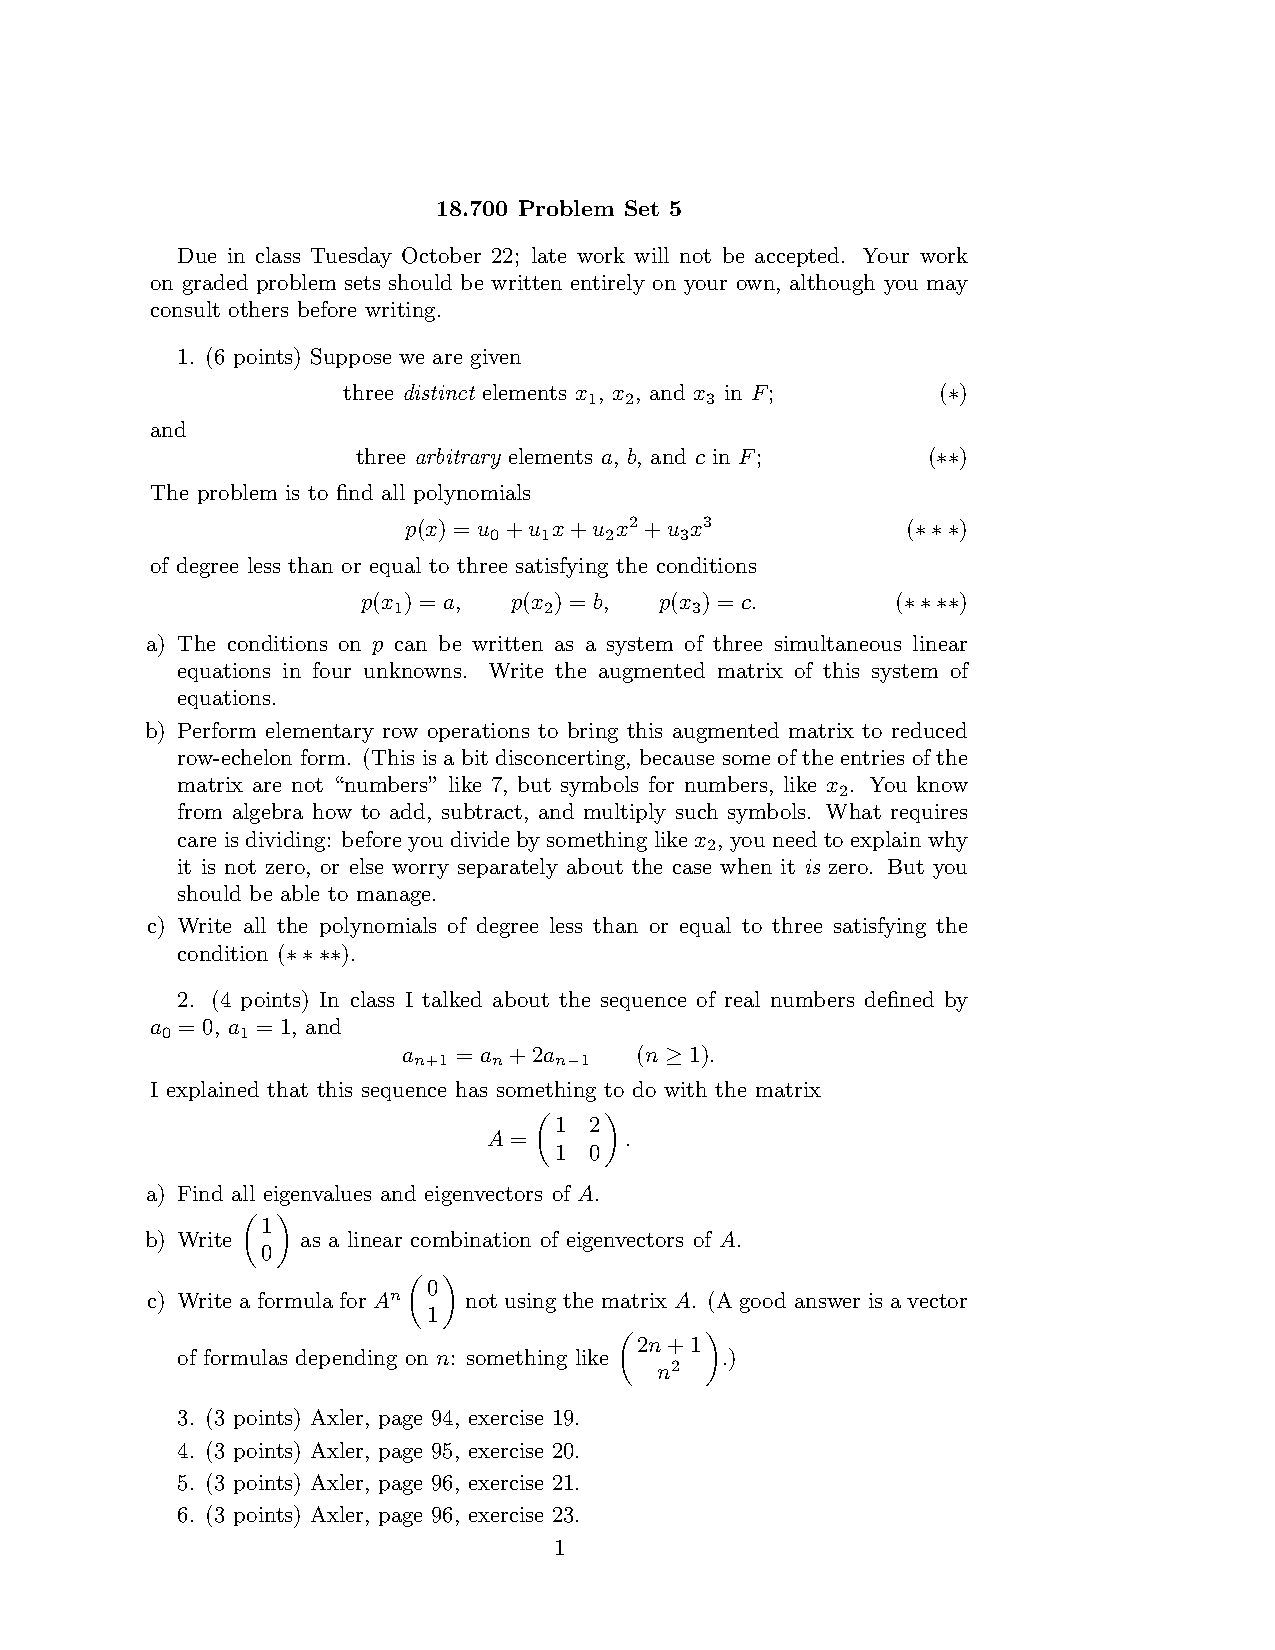
\includepdf[link=true, linkname=LinearAlgebra-ProblemSet5,pages=1]{MIT/Problems/18.700/ProblemSet5.pdf}
\section*{Question 1}
\subsection*{Part a}
\begin{eqnarray*}
\left(\begin{array}{rrrr|r}
1 & x_{1} & x_{1}^{2} & x_{1}^{3} & a \\
1 & x_{2} & x_{2}^{2} & x_{2}^{3} & b \\
1 & x_{3} & x_{3}^{2} & x_{3}^{3} & c
\end{array}\right)
\end{eqnarray*}
\subsection*{Part b}
Here we start:
\begin{eqnarray*}
\left(\begin{array}{rrrr|r}
1 & x_{1} & x_{1}^{2} & x_{1}^{3} & a \\
1 & x_{2} & x_{2}^{2} & x_{2}^{3} & b \\
1 & x_{3} & x_{3}^{2} & x_{3}^{3} & c
\end{array}\right)
\end{eqnarray*}
Subtract the second row by the first.
\begin{eqnarray*}
\left(\begin{array}{rrrr|r}
1 & x_{1} & x_{1}^{2} & x_{1}^{3} & a \\
0 & -x_{1} + x_{2} & -x_{1}^{2} + x_{2}^{2} & -x_{1}^{3} + x_{2}^{3} & -a + b \\
1 & x_{3} & x_{3}^{2} & x_{3}^{3} & c
\end{array}\right)
\end{eqnarray*}
We introduced some difference of powers, they can be factorized.
\begin{eqnarray*}
\left(\begin{array}{rrrr|r}
1 & x_{1} & x_{1}^{2} & x_{1}^{3} & a \\
0 & -x_{1} + x_{2} & -{\left(x_{1} + x_{2}\right)} {\left(x_{1} - x_{2}\right)} & -{\left(x_{1}^{2} + x_{1} x_{2} + x_{2}^{2}\right)} {\left(x_{1} - x_{2}\right)} & -a + b \\
1 & x_{3} & x_{3}^{2} & x_{3}^{3} & c
\end{array}\right)
\end{eqnarray*}
Subtract the third row by the first.
\begin{eqnarray*}
\left(\begin{array}{rrrr|r}
1 & x_{1} & x_{1}^{2} & x_{1}^{3} & a \\
0 & -x_{1} + x_{2} & -{\left(x_{1} + x_{2}\right)} {\left(x_{1} - x_{2}\right)} & -{\left(x_{1}^{2} + x_{1} x_{2} + x_{2}^{2}\right)} {\left(x_{1} - x_{2}\right)} & -a + b \\
0 & -x_{1} + x_{3} & -x_{1}^{2} + x_{3}^{2} & -x_{1}^{3} + x_{3}^{3} & -a + c
\end{array}\right)
\end{eqnarray*}
Again, we have some difference of powers, they can be factorized as well.
\begin{eqnarray*}
\left(\begin{array}{rrrr|r}
1 & x_{1} & x_{1}^{2} & x_{1}^{3} & a \\
0 & -x_{1} + x_{2} & -{\left(x_{1} + x_{2}\right)} {\left(x_{1} - x_{2}\right)} & -{\left(x_{1}^{2} + x_{1} x_{2} + x_{2}^{2}\right)} {\left(x_{1} - x_{2}\right)} & -a + b \\
0 & -x_{1} + x_{3} & -{\left(x_{1} + x_{3}\right)} {\left(x_{1} - x_{3}\right)} & -{\left(x_{1}^{2} + x_{1} x_{3} + x_{3}^{2}\right)} {\left(x_{1} - x_{3}\right)} & -a + c
\end{array}\right)
\end{eqnarray*}
With the factorization, we can easily scale down the second row.
\begin{eqnarray*}
\left(\begin{array}{rrrr|r}
1 & x_{1} & x_{1}^{2} & x_{1}^{3} & a \\
0 & 1 & x_{1} + x_{2} & x_{1}^{2} + x_{1} x_{2} + x_{2}^{2} & \frac{a - b}{x_{1} - x_{2}} \\
0 & -x_{1} + x_{3} & -{\left(x_{1} + x_{3}\right)} {\left(x_{1} - x_{3}\right)} & -{\left(x_{1}^{2} + x_{1} x_{3} + x_{3}^{2}\right)} {\left(x_{1} - x_{3}\right)} & -a + c
\end{array}\right)
\end{eqnarray*}
And scale down the third row as well
\begin{eqnarray*}
\left(\begin{array}{rrrr|r}
1 & x_{1} & x_{1}^{2} & x_{1}^{3} & a \\
0 & 1 & x_{1} + x_{2} & x_{1}^{2} + x_{1} x_{2} + x_{2}^{2} & \frac{a - b}{x_{1} - x_{2}} \\
0 & 1 & x_{1} + x_{3} & x_{1}^{2} + x_{1} x_{3} + x_{3}^{2} & \frac{a - c}{x_{1} - x_{3}}
\end{array}\right)
\end{eqnarray*}
Subtract the first row by the second row multiplied by $ x_1 $ times.
\begin{eqnarray*}
\left(\begin{array}{rrrr|r}
1 & 0 & -{\left(x_{1} + x_{2}\right)} x_{1} + x_{1}^{2} & x_{1}^{3} - {\left(x_{1}^{2} + x_{1} x_{2} + x_{2}^{2}\right)} x_{1} & a - \frac{{\left(a - b\right)} x_{1}}{x_{1} - x_{2}} \\
0 & 1 & x_{1} + x_{2} & x_{1}^{2} + x_{1} x_{2} + x_{2}^{2} & \frac{a - b}{x_{1} - x_{2}} \\
0 & 1 & x_{1} + x_{3} & x_{1}^{2} + x_{1} x_{3} + x_{3}^{2} & \frac{a - c}{x_{1} - x_{3}}
\end{array}\right)
\end{eqnarray*}
Note that we could cancel some terms if we expand it.
\begin{eqnarray*}
\left(\begin{array}{rrrr|r}
1 & 0 & -x_{1} x_{2} & -x_{1}^{2} x_{2} - x_{1} x_{2}^{2} & a - \frac{{\left(a - b\right)} x_{1}}{x_{1} - x_{2}} \\
0 & 1 & x_{1} + x_{2} & x_{1}^{2} + x_{1} x_{2} + x_{2}^{2} & \frac{a - b}{x_{1} - x_{2}} \\
0 & 1 & x_{1} + x_{3} & x_{1}^{2} + x_{1} x_{3} + x_{3}^{2} & \frac{a - c}{x_{1} - x_{3}}
\end{array}\right)
\end{eqnarray*}
Subtract the third row by the second row.
\begin{eqnarray*}
\left(\begin{array}{rrrr|r}
1 & 0 & -x_{1} x_{2} & -x_{1}^{2} x_{2} - x_{1} x_{2}^{2} & \frac{b x_{1} - a x_{2}}{x_{1} - x_{2}} \\
0 & 1 & x_{1} + x_{2} & x_{1}^{2} + x_{1} x_{2} + x_{2}^{2} & \frac{a - b}{x_{1} - x_{2}} \\
0 & 0 & -x_{2} + x_{3} & -x_{1} x_{2} - x_{2}^{2} + x_{1} x_{3} + x_{3}^{2} & \frac{b x_{1} - c x_{1} - a x_{2} + c x_{2} + a x_{3} - b x_{3}}{{\left(x_{1} - x_{2}\right)} {\left(x_{1} - x_{3}\right)}}
\end{array}\right)
\end{eqnarray*}
While it is not very clear, we can actually factorize the row 3 
\begin{eqnarray*}
\left(\begin{array}{rrrr|r}
1 & 0 & -x_{1} x_{2} & -x_{1}^{2} x_{2} - x_{1} x_{2}^{2} & \frac{b x_{1} - a x_{2}}{x_{1} - x_{2}} \\
0 & 1 & x_{1} + x_{2} & x_{1}^{2} + x_{1} x_{2} + x_{2}^{2} & \frac{a - b}{x_{1} - x_{2}} \\
0 & 0 & -x_{2} + x_{3} & -{\left(x_{1} + x_{2} + x_{3}\right)} {\left(x_{2} - x_{3}\right)} & \frac{b x_{1} - c x_{1} - a x_{2} + c x_{2} + a x_{3} - b x_{3}}{{\left(x_{1} - x_{2}\right)} {\left(x_{1} - x_{3}\right)}}
\end{array}\right)
\end{eqnarray*}
Now we can easily scale down row 3 after the factorization
\begin{eqnarray*}
\left(\begin{array}{rrrr|r}
1 & 0 & -x_{1} x_{2} & -x_{1}^{2} x_{2} - x_{1} x_{2}^{2} & \frac{b x_{1} - a x_{2}}{x_{1} - x_{2}} \\
0 & 1 & x_{1} + x_{2} & x_{1}^{2} + x_{1} x_{2} + x_{2}^{2} & \frac{a - b}{x_{1} - x_{2}} \\
0 & 0 & 1 & x_{1} + x_{2} + x_{3} & -\frac{b x_{1} - c x_{1} - a x_{2} + c x_{2} + a x_{3} - b x_{3}}{{\left(x_{1} - x_{2}\right)} {\left(x_{1} - x_{3}\right)} {\left(x_{2} - x_{3}\right)}}
\end{array}\right)
\end{eqnarray*}
Subtract the second row by the third row multiplied by $ x_1 + x_2 $ times.
\begin{eqnarray*}
\left(\begin{array}{rrrr|r}
1 & 0 & -x_{1} x_{2} & -x_{1}^{2} x_{2} - x_{1} x_{2}^{2} & \frac{b x_{1} - a x_{2}}{x_{1} - x_{2}} \\
0 & 1 & 0 & -{\left(x_{1} + x_{2} + x_{3}\right)} {\left(x_{1} + x_{2}\right)} + x_{1}^{2} + x_{1} x_{2} + x_{2}^{2} & \frac{b x_{1}^{2} - c x_{1}^{2} - a x_{2}^{2} + c x_{2}^{2} + a x_{3}^{2} - b x_{3}^{2}}{{\left(x_{1} - x_{2}\right)} {\left(x_{1} - x_{3}\right)} {\left(x_{2} - x_{3}\right)}} \\
0 & 0 & 1 & x_{1} + x_{2} + x_{3} & -\frac{b x_{1} - c x_{1} - a x_{2} + c x_{2} + a x_{3} - b x_{3}}{{\left(x_{1} - x_{2}\right)} {\left(x_{1} - x_{3}\right)} {\left(x_{2} - x_{3}\right)}}
\end{array}\right)
\end{eqnarray*}
Observe that some terms cancel if we expand the product
\begin{eqnarray*}
\left(\begin{array}{rrrr|r}
1 & 0 & -x_{1} x_{2} & -x_{1}^{2} x_{2} - x_{1} x_{2}^{2} & \frac{b x_{1} - a x_{2}}{x_{1} - x_{2}} \\
0 & 1 & 0 & -x_{1} x_{2} - x_{1} x_{3} - x_{2} x_{3} & \frac{b x_{1}^{2} - c x_{1}^{2} - a x_{2}^{2} + c x_{2}^{2} + a x_{3}^{2} - b x_{3}^{2}}{{\left(x_{1} - x_{2}\right)} {\left(x_{1} - x_{3}\right)} {\left(x_{2} - x_{3}\right)}} \\
0 & 0 & 1 & x_{1} + x_{2} + x_{3} & -\frac{b x_{1} - c x_{1} - a x_{2} + c x_{2} + a x_{3} - b x_{3}}{{\left(x_{1} - x_{2}\right)} {\left(x_{1} - x_{3}\right)} {\left(x_{2} - x_{3}\right)}}
\end{array}\right)
\end{eqnarray*}
Add the first row by the third row multiplied by $ x_1 x_2 $ times.
\begin{eqnarray*}
\left(\begin{array}{rrrr|r}
1 & 0 & 0 & {\left(x_{1} + x_{2} + x_{3}\right)} x_{1} x_{2} - x_{1}^{2} x_{2} - x_{1} x_{2}^{2} & \frac{c x_{1}^{2} x_{2} - c x_{1} x_{2}^{2} - b x_{1}^{2} x_{3} + a x_{2}^{2} x_{3} + b x_{1} x_{3}^{2} - a x_{2} x_{3}^{2}}{{\left(x_{1} - x_{2}\right)} {\left(x_{1} - x_{3}\right)} {\left(x_{2} - x_{3}\right)}} \\
0 & 1 & 0 & -x_{1} x_{2} - x_{1} x_{3} - x_{2} x_{3} & \frac{b x_{1}^{2} - c x_{1}^{2} - a x_{2}^{2} + c x_{2}^{2} + a x_{3}^{2} - b x_{3}^{2}}{{\left(x_{1} - x_{2}\right)} {\left(x_{1} - x_{3}\right)} {\left(x_{2} - x_{3}\right)}} \\
0 & 0 & 1 & x_{1} + x_{2} + x_{3} & -\frac{b x_{1} - c x_{1} - a x_{2} + c x_{2} + a x_{3} - b x_{3}}{{\left(x_{1} - x_{2}\right)} {\left(x_{1} - x_{3}\right)} {\left(x_{2} - x_{3}\right)}}
\end{array}\right)
\end{eqnarray*}
Again, observe that some terms cancel if we expand the product
\begin{eqnarray*}
\left(\begin{array}{rrrr|r}
1 & 0 & 0 & x_{1} x_{2} x_{3} & \frac{c x_{1}^{2} x_{2} - c x_{1} x_{2}^{2} - b x_{1}^{2} x_{3} + a x_{2}^{2} x_{3} + b x_{1} x_{3}^{2} - a x_{2} x_{3}^{2}}{{\left(x_{1} - x_{2}\right)} {\left(x_{1} - x_{3}\right)} {\left(x_{2} - x_{3}\right)}} \\
0 & 1 & 0 & -x_{1} x_{2} - x_{1} x_{3} - x_{2} x_{3} & \frac{b x_{1}^{2} - c x_{1}^{2} - a x_{2}^{2} + c x_{2}^{2} + a x_{3}^{2} - b x_{3}^{2}}{{\left(x_{1} - x_{2}\right)} {\left(x_{1} - x_{3}\right)} {\left(x_{2} - x_{3}\right)}} \\
0 & 0 & 1 & x_{1} + x_{2} + x_{3} & -\frac{b x_{1} - c x_{1} - a x_{2} + c x_{2} + a x_{3} - b x_{3}}{{\left(x_{1} - x_{2}\right)} {\left(x_{1} - x_{3}\right)} {\left(x_{2} - x_{3}\right)}}
\end{array}\right)
\end{eqnarray*}
Observe that we have a very nice symmetric left hand side while the right hand side is a mess. The issue is that $ a, b, c $ make the problem asymmetric, and they are all concentrated at the last column, that is why that column looks particular complicated.

Doing these tedious manipulation is very error prone, and therefore it is best left for the computer. Sage is capable to produce a reduced echelon form directly, but it make questionable division and produced a matrix that is very complicated. In order to reach this relatively simple form, I need to guide it to do the right simplification at the right time. For the record, here is the code used to produce the \LaTeX above. 
\begin{verbatim}
%typeset_mode True

p = var("x_1")
q = var("x_2")
r = var("x_3")
a = var("a")
b = var("b")
c = var("c")
l1 = Matrix([[1,p,p^2,p^3],[1,q,q^2,q^3],[1,r,r^2,r^3]])
r1 = Matrix([[a],[b],[c]])

print("Here we start:")
print("\\begin{eqnarray*}")
latex(l1.augment(r1))
print("\\end{eqnarray*}")

l2 = l1.with_added_multiple_of_row(1,0,-1)
r2 = r1.with_added_multiple_of_row(1,0,-1).factor().simplify()

print("Subtract the second row by the first.")
print("\\begin{eqnarray*}")
latex(l2.augment(r2))
print("\\end{eqnarray*}")

l3 = l2
r3 = r2
l3[1,2] = l3[1,2].factor()
l3[1,3] = l3[1,3].factor()

print("We introduced some difference of powers, they can be factorized.")
print("\\begin{eqnarray*}")
latex(l3.augment(r3))
print("\\end{eqnarray*}")

l4 = l3.with_added_multiple_of_row(2,0,-1)
r4 = r3.with_added_multiple_of_row(2,0,-1).factor().simplify()

print("Subtract the third row by the first.")
print("\\begin{eqnarray*}")
latex(l4.augment(r4))
print("\\end{eqnarray*}")

l5 = l4
r5 = r4
l5[2,2] = l5[2,2].factor()
l5[2,3] = l5[2,3].factor()

print("Again, we have some difference of powers, they can be factorized as well.")
print("\\begin{eqnarray*}")
latex(l5.augment(r5))
print("\\end{eqnarray*}")

l6 = l5.with_rescaled_row(1,1/(q-p))
r6 = r5.with_rescaled_row(1,1/(q-p)).factor().simplify()

print("With the factorization, we can easily scale down the second row.")
print("\\begin{eqnarray*}")
latex(l6.augment(r6))
print("\\end{eqnarray*}")

l7 = l6.with_rescaled_row(2,1/(r-p))
r7 = r6.with_rescaled_row(2,1/(r-p)).factor().simplify()

print("And scale down the third row as well")
print("\\begin{eqnarray*}")
latex(l7.augment(r7))
print("\\end{eqnarray*}")

l8 = l7.with_added_multiple_of_row(0,1,-p)
r8 = r7.with_added_multiple_of_row(0,1,-p)

print("Subtract the first row by the second row multiplied by $ x_1 $ times.")
print("\\begin{eqnarray*}")
latex(l8.augment(r8))
print("\\end{eqnarray*}")

l9 = l8
r9 = r8
l9[0,2] = l9[0,2].expand().simplify()
l9[0,3] = l9[0,3].expand().simplify()

print("Note that we could cancel some terms if we expand it.")
print("\\begin{eqnarray*}")
latex(l9.augment(r9))
print("\\end{eqnarray*}")

l10 = l9.with_added_multiple_of_row(2,1,-1)
r10 = r9.with_added_multiple_of_row(2,1,-1).factor().simplify()

print("Subtract the third row by the second row.")
print("\\begin{eqnarray*}")
latex(l10.augment(r10))
print("\\end{eqnarray*}")

l11 = l10
r11 = r10
l11[2,3] = l11[2,3].factor()

print("While it is not very clear, we can actually factorize the row 3 ")
print("\\begin{eqnarray*}")
latex(l11.augment(r11))
print("\\end{eqnarray*}")

l12 = l11.with_rescaled_row(2,1/(r-q))
r12 = r11.with_rescaled_row(2,1/(r-q)).factor().simplify()

print("Now we can easily scale down row 3 after the factorization")
print("\\begin{eqnarray*}")
latex(l12.augment(r12))
print("\\end{eqnarray*}")

l13 = l12.with_added_multiple_of_row(1,2,-p-q)
r13 = r12.with_added_multiple_of_row(1,2,-p-q).factor().simplify()

print("Subtract the second row by the third row multiplied by $ x_1 + x_2 $ times.")
print("\\begin{eqnarray*}")
latex(l13.augment(r13))
print("\\end{eqnarray*}")

l14 = l13
r14 = r13
l14[1,3] = l14[1,3].expand().simplify()

print("Observe that some terms cancel if we expand the product")
print("\\begin{eqnarray*}")
latex(l14.augment(r14))
print("\\end{eqnarray*}")

l15 = l14.with_added_multiple_of_row(0,2,p*q)
r15 = r14.with_added_multiple_of_row(0,2,p*q).factor().simplify()

print("Add the first row by the third row multiplied by $ x_1 x_2 $ times.")
print("\\begin{eqnarray*}")
latex(l15.augment(r15))
print("\\end{eqnarray*}")

l16 = l15
r16 = r15
l16[0,3] = l16[0,3].expand().simplify()

print("Again, observe that some terms cancel if we expand the product")
print("\\begin{eqnarray*}")
latex(l16.augment(r16))
print("\\end{eqnarray*}")
\end{verbatim}
Even with computer, this is taking me a lot of hours, and this is a bad approach to solve this problem, as we will see in the next part.
\subsection*{Part c}
We can easily find a polynomial satisfying the constraint using Lagrange's interpolation as follow:
\begin{eqnarray*}
    \frac{(x - x_2)(x - x_3)}{(x_1 - x_2)(x_1 - x_3)} a + \frac{(x - x_1)(x - x_3)}{(x_2 - x_1)(x_2 - x_3)} b + \frac{(x - x_1)(x - x_2)}{(x_3 - x_1)(x_3 - x_2)} c
\end{eqnarray*}
Now suppose we have two such polynomials $ f $ and $ g $. we notice that $ f - g $ must have three roots at $ \{ x_1, x_2, x_3\} $, that means $ f - g = n(x - x_1)(x-x_2)(x - x_3) $ for an arbitrary $ n \in F $.

So the solution is simply 
\begin{eqnarray*}
    \frac{(x - x_2)(x - x_3)}{(x_1 - x_2)(x_1 - x_3)} a + \frac{(x - x_1)(x - x_3)}{(x_2 - x_1)(x_2 - x_3)} b + \frac{(x - x_1)(x - x_2)}{(x_3 - x_1)(x_3 - x_2)} c + n(x - x_1)(x-x_2)(x - x_3)
\end{eqnarray*}

Note how this solution ressemble the reduced echelon form we found in part b. The denominator on the right hand side comes from the Lagrange interpolation, and the symmetric polynomials on the left hand side comes from the expansion of  $ (x - x_1)(x-x_2)(x - x_3) $. This also shows the solution lies in a one dimensional subspace of $ F_4 $, which also agree with the reduced echelon form.

\end{document}
